\documentclass[../Head/Main.tex]{subfiles}
\begin{document}
\subsection{Motion planers in action}
\label{subsec:testMotionPlanning}

The purpose of this test is to find out how well the motion planners work in an actual environment with obstacles. The goal is to lead the robot from an initial position to a target location. 

\subsubsection*{Description of test}

The initial position of the robot will be in the origin of the environment of the gazebo simulator. Here 14 test of both the tangent bug algorithm and model based planner was conducted for the 14 rooms of the bigworld map. The idea is to test the success rate of finding rooms, the robots distance to the closest obstacle on the path to the goal and the distance travelled along the way. The model based planer will be tested with a higher speed than the tangent bug algorithm because it will be further away from obstacle most of the time and thereby less likely of hitting obstacles.           

\subsubsection*{Test parameters}

\begin{tabular}{l r l}
	- World used                    & bigworld & \\	
	- Velocity of tangent bug       & $U=\{-1~to~1\}$ & (Universe of discourse)\\
	- Velocity of model planner     & $U=\{-2~to~2\}$ & (Universe of discourse)\\
	- Number of tests               & 14 & 
\end{tabular}

\subsubsection*{Data}

If one compares the model based planner in table (\ref{tab:modelbased}) with the sensor based planner in table (\ref{tab:sensorbased}) many observations is observed. The model based planner has a success rate of finding rooms at 100 \% with and average travelled distance of 46.9 meters. Compared to the sensor based planner with a success rate of 64.3 \% and average distance on 27.9 meters, the model based performs very well in finding rooms, but it comes with a cost of distance travelled compared to the sensor based. It is clear from figure (\ref{fig:Test9}) that when the sensor based planner performs well, it outperforms the model based planner in distance travelled.    

\begin{table}[H]
	\subfile{../Tables/Dist_travelled_and_dist_to_obstacle_modelbased}
	\caption{Table over test data for the model based planner}
	\label{tab:modelbased}
\end{table}

\begin{table}[H]
	\subfile{../Tables/Dist_travelled_and_dist_to_obstacle_tangent_bug}
	\caption{Table over test data for the sensor based planner}
	\label{tab:sensorbased}
\end{table}


\subfile{../Figures/Graphs_dist_to_obstacle}
\subfile{../Figures/Comparason_motion_planners}

\begin{figure}[H]
	\centering
	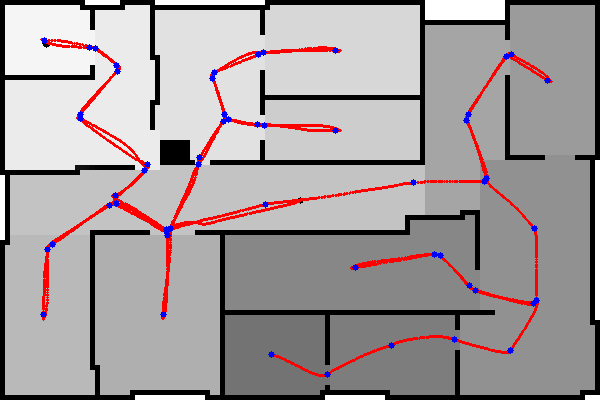
\includegraphics[width=0.6\textwidth]{Modelbased/brushfireTest15}
	\caption{Illustration of the run visiting all rooms starting from the origin for the model based planner}
	\label{fig:Test15}
\end{figure}

\subsubsection*{Conclusion}

The model based planner is more reliable than the sensor based planner in that it has a success rate of finding rooms at 100 \% compared to 64.3 \% for the sensor based. However the sensor based planner has an average distance travelled about 27.9 meters compared to the model based about 46.9 meters. It can therefore be concluded that the sensor based planner outperforms the model based in certain scenarios, but the model based is more reliable in finding rooms. 

\end{document}